\documentclass[12pt]{article}

\usepackage[margin=1in]{geometry}
\usepackage{amsmath}
\usepackage{biblatex}
\usepackage{parskip}
\usepackage{graphicx}
\usepackage{float}
\usepackage{fancyhdr}
\usepackage{lastpage}
\usepackage{titlesec}
\usepackage{enumitem}
\usepackage{subfig}
\usepackage{hyperref}
\usepackage{soul}

\pagestyle{fancy}
\renewcommand{\headrulewidth}{0pt}
\renewcommand{\footrulewidth}{0pt}
\fancyhf{}
\lfoot{\scriptsize January 2019}
\cfoot{\scriptsize Brendon Matusch---Improving Particle Classification in WIMP Experiments}
\rfoot{\scriptsize Page~\thepage~of~\pageref{LastPage}}

\graphicspath{{./images/}}

\addbibresource{paper.bib}

\titlespacing{\section}{0pt}{0pt}{0pt}
\titlespacing{\subsection}{0pt}{0pt}{0pt}
\titlespacing{\subsubsection}{0pt}{0pt}{0pt}

\titleformat*{\section}{\large\bfseries}
\titleformat*{\subsection}{\normalsize\bfseries}
\titleformat*{\subsubsection}{\normalsize\bfseries}

\begin{document}

\begin{center}
    \begin{Large}
        Improving Particle Classification in WIMP Dark Matter Detection Experiments Using Neural Networks
    \end{Large}

    Brendon Matusch
\end{center}

\section{Introduction}

In all experiments for detection of WIMP dark matter, it is essential to develop a classifier that can distinguish WIMP events from background radiation, in particular alpha particles. Manually developing such a classifier necessitates time-consuming physical modeling.

Machine learning (ML) has the potential to automate this and accelerate experimentation, and also to detect patterns that humans cannot. However, impure calibration data hinders training of models, and unusual detector topologies make data challenging to process.

I worked with two dark matter experiments: the PICO-60 bubble chamber \cite{pico}, and the DEAP-3600 liquid argon scintillator \cite{deap}. In PICO-60, background alpha and WIMP-like neutron calibration datasets are used for training; however, there is an impurity of 10\% alphas in the neutron set, hindering training. In DEAP-3600, the detector format, containing 255 spherically arranged photomultiplier tubes (PMTs), makes data processing challenging.

Previously in PICO-60, a conventional classifier was developed and is thought to be 100\% accurate. However, machine learning is also applicable because it is quicker to develop and re-calibrate. A supervised neural network was used, reaching a mean of 80.2\% accuracy.

In DEAP-3600, a simulation was developed prior to my work, because it is impractical to collect large amounts of calibration data. A conventional classifier removes 99.6\% of alpha background radiation, while also (undesirably) removing 91.0\% of simulated WIMP events.

My objective was to develop novel machine learning algorithms that are more accurate, and I succeeded at this goal! I composed a 28-page research whitepaper \cite{me} about my work on PICO-60, which has been reviewed and approved by the PICO collaboration and pre-published at \url{https://arxiv.org/abs/1811.11308}. It is currently undergoing peer review for eventual publication in the journal \textit{Computer Physics Communications}.

\ul{Please note that the entire PICO collaboration are listed on the research whitepaper because of their contributions to the original PICO-60 dark matter experiment. They did not contribute to this study; I completed and documented it independently.}

\section{Procedure}

\subsection{PICO-60}

For PICO-60, I developed and compared two sets of classification algorithms: supervised learning, and semi-supervised learning.

\subsubsection{Supervised Learning}

I experimented further with supervised learning, exploring the following data formats to learn which was the best-performing solution:

\begin{enumerate}
    \item An 8-band Fourier transform of audio recorded in the bubble chamber. I applied a dense neural network with dropout \cite{dropout} and L2 regularization (which allowed for less overfitting to impure data).
    \item A full-resolution Fourier transform of the audio (all 50,001 data points). I once again applied a dense neural network with the Adam \cite{adam} optimizer.
    \item A raw audio waveform with a very deep 1D convolutional neural network (CNN) inspired by Dai et al.\ \cite{verydeepconvnets}.
    \item Images captured by cameras in the detector. I trained a 2D CNN on these, to learn whether they contain any relevant information.
\end{enumerate}

\begin{figure}[ht]
    \centering
    \subfloat{\fbox{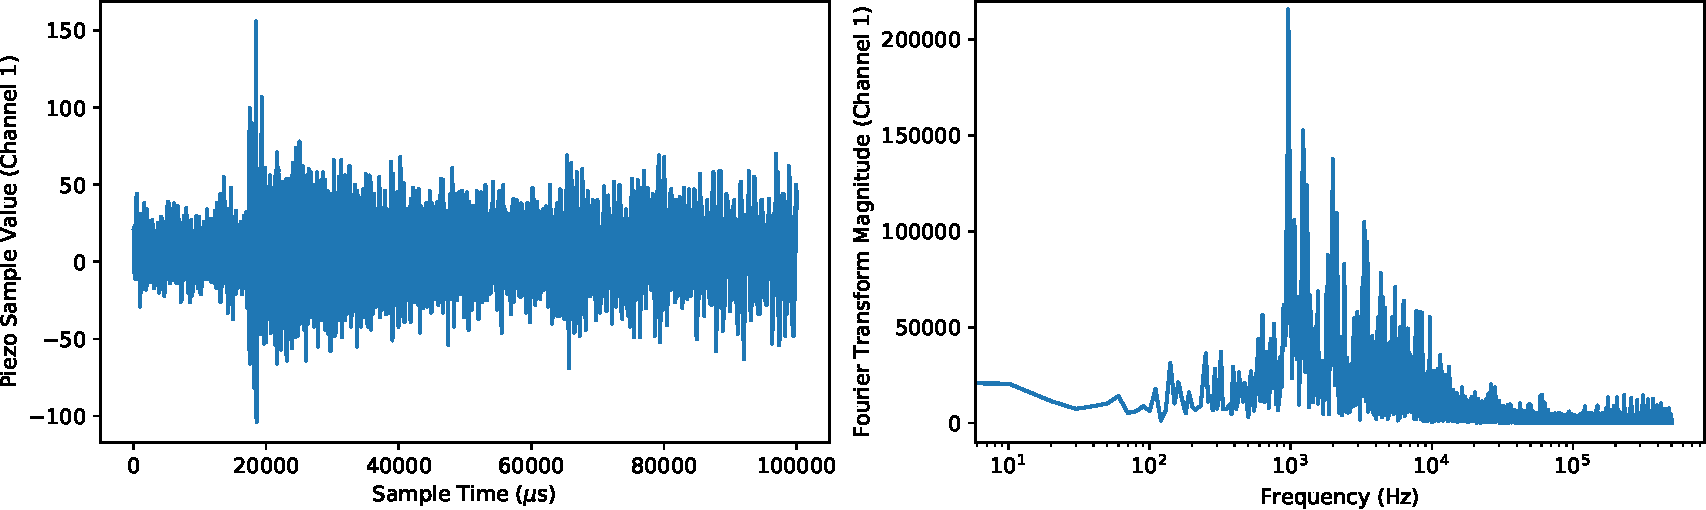
\includegraphics[width=0.8\textwidth]{audio_cropped}}}
    \qquad
    \subfloat{\fbox{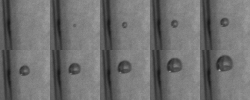
\includegraphics[width=0.45\textwidth]{image_grid}}}
    \caption{Examples of the audio waveform and Fourier transform (above) and the images captured by cameras (below).}
\end{figure}

\subsubsection{Semi-Supervised Learning}

To even better handle impurities, I developed two novel semi-supervised learning algorithms. The impure alpha/WIMP-like labels were removed from a large portion of the training data, and my algorithms learned more accurate labels for this data.

\begin{enumerate}
    \item Iterative Cluster Nucleation is inspired by unsupervised clustering algorithms, and takes advantage of the ``confidence'' of the neural network's predictions (that is, how close the predictions are to 0 or 1).
    
    First, a neural network is trained on a labeled set. After 30 epochs, it runs predictions on the unlabeled set. As the network trains, the confidence of these predictions increases. When $p < t$ or $p > 1 - t$ for a given prediction $p$ and a (small) confidence threshold $t$, the example is labeled correspondingly and added to the labeled set.

    It is hypothesized that accuracy will gradually \textit{improve} as the neural network's most confident predictions are fed back into the network as newly labeled training data.

    \item Gravitational Differentiation is an analog alternative to Iterative Cluster Nucleation. Using a novel piecewise exponential function for calculating final-layer derivatives, called $\mathrm{GravDiff}(p, \psi, g)$, unlabeled examples are caused to "gravitate" toward more accurate predictions based on the confidence of the neural network's predictions.

    The function is a transformation of the hyperbolic tangent that flattens the central range and comparatively exaggerates the asymptote on either side, defined as follows:
    \begin{center}
        $\mathrm{GravDiff}(p, \psi, g) = g \cdot \mathrm{sgn}(p) \cdot \lvert \mathrm{tanh}(2p - 1) \rvert ^ \psi$
    \end{center}
    where $p$ is the network's prediction, $\psi$ determines the rate at which the output approaches 0 as the confidence of the prediction decreases, and $g$ is the learning rate multiplier. The output is the final-layer gradient to be used in backpropagation.
\end{enumerate}

\subsection{DEAP-3600}

In DEAP-3600, the key challenge is the aforementioned unusual detector format: a sphere (with an opening on the top) tiled with a hexagonal lattice of PMTs. I approached this problem in three different ways:

\begin{enumerate}
    \item I tried simply inputting photon counts from each PMT into a multi-layer perceptron.

    \item I developed and applied a Mercator-like cylindrical projection, which maps a sphere onto a rectangle. Cubic spline interpolation was used to map latitude lines on the sphere (which vary in length) to equal-length rows on the rectangular image.

    \item I developed a new type of CNN, called a topological CNN. Rather than a 2D image of square pixels, kernels convolve over an arbitrary topology.
    
    While a conventional convolutional layer downscales a rectangular image to a smaller rectangular image by multiplying square regions by a set of corresponding weights, a topological CNN (as applied to this problem) downscales the approximately spherical hexagonal mesh to a smaller but topologically equivalent hexagonal mesh.
\end{enumerate}

\begin{figure}[ht]
    \centering
    \fbox{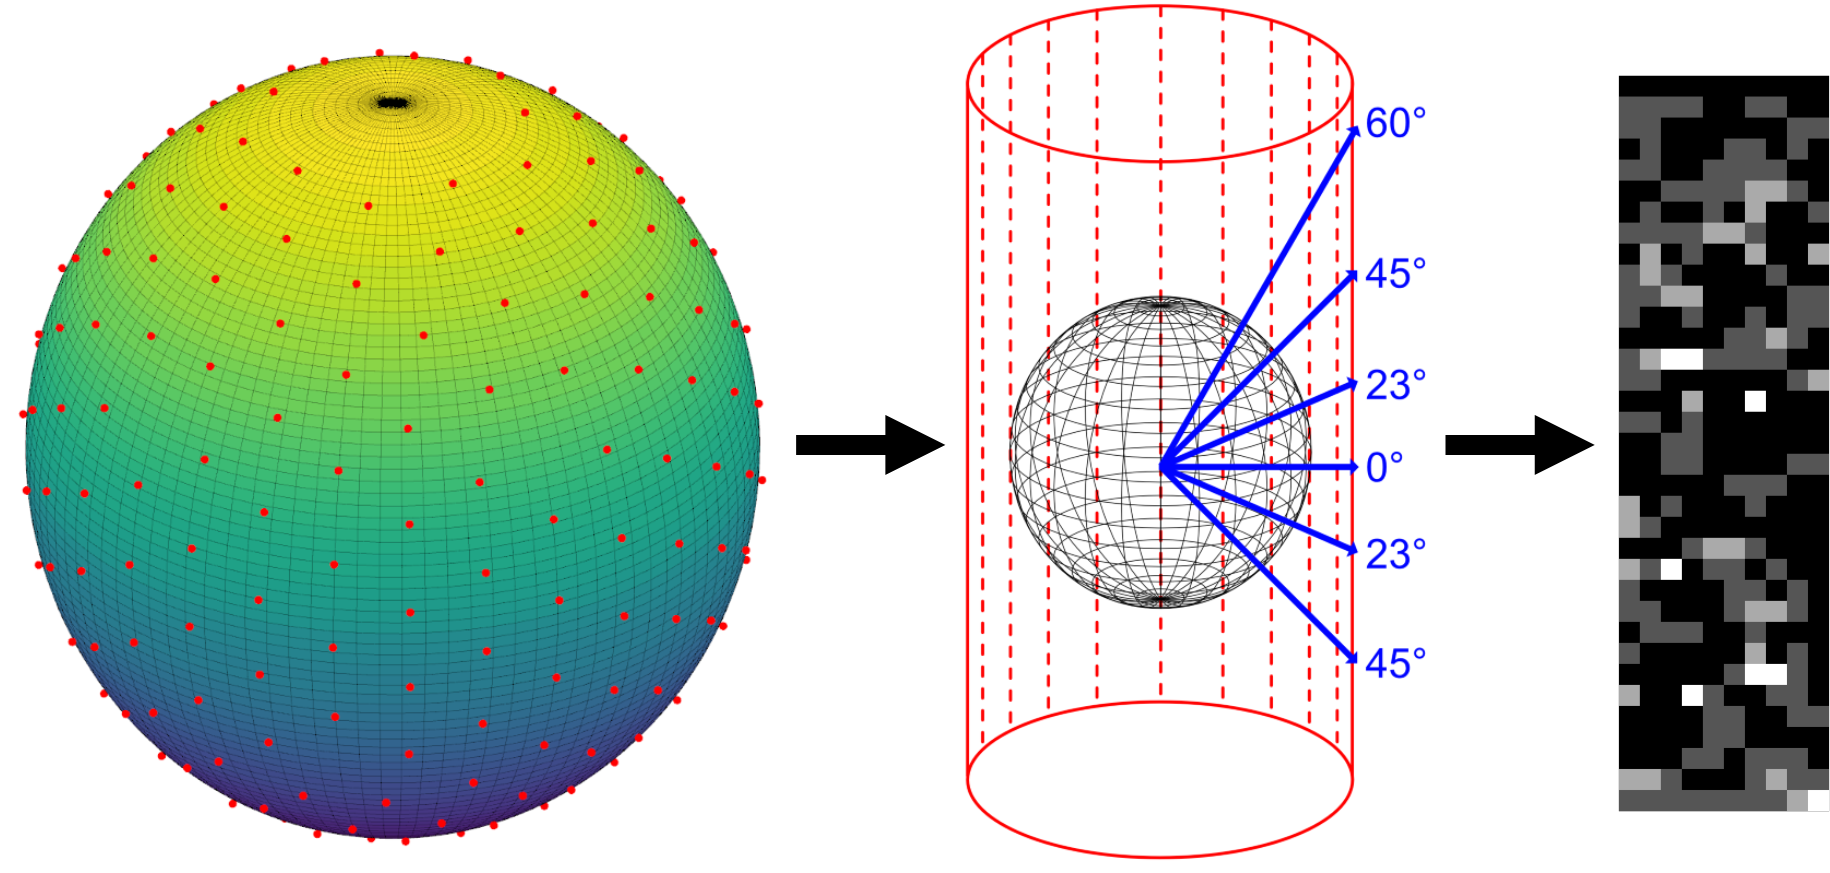
\includegraphics[width=0.45\textwidth]{map_projection}}
    \qquad
    \fbox{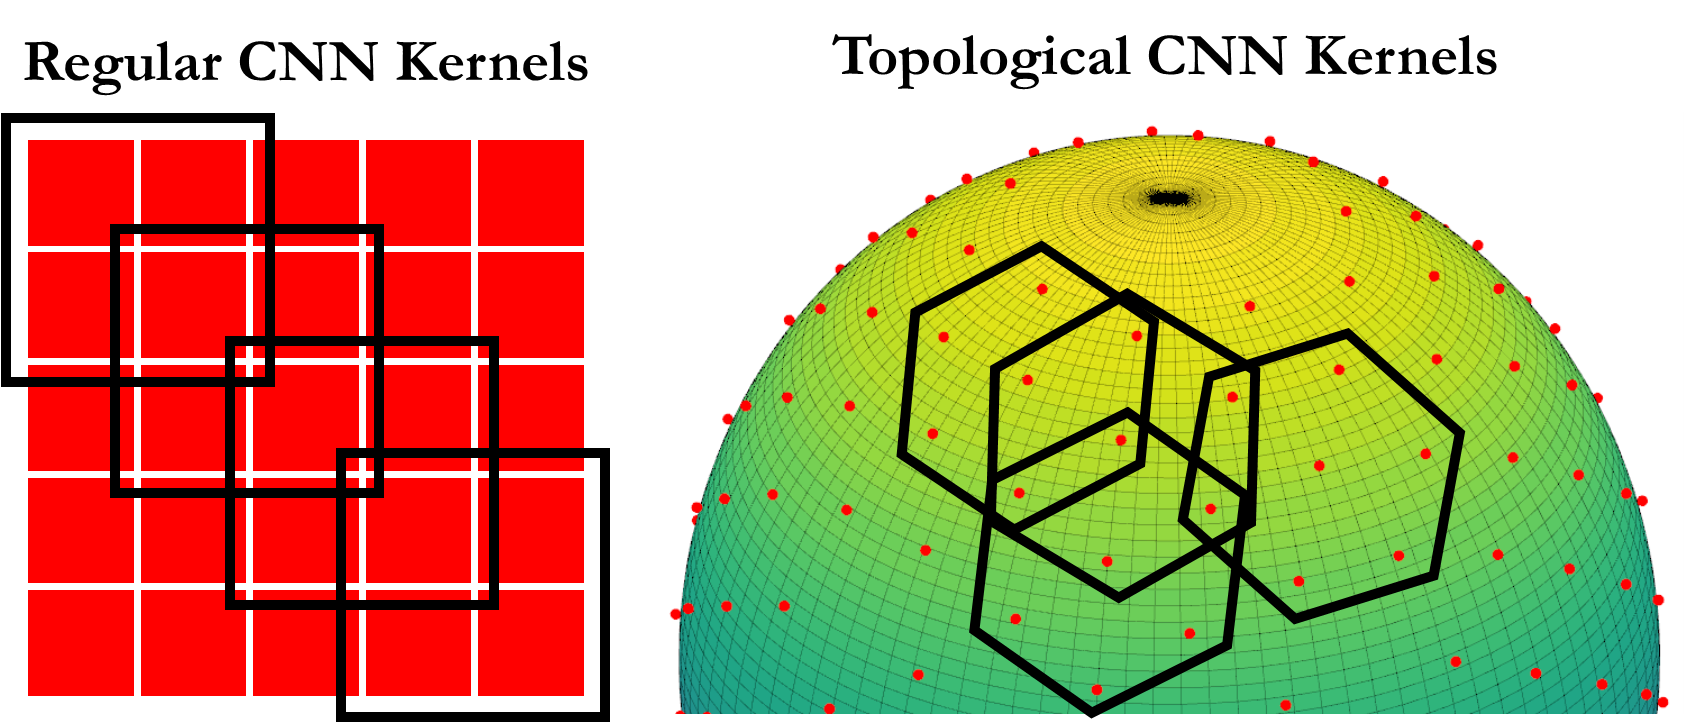
\includegraphics[width=0.45\textwidth]{topological}}
    \caption{Diagrams of the cylindrical projection (left) and topological CNN (right) systems.}
\end{figure}

\subsection{Statistical Practices}

Models were optimized using grid searches, in which every configuration within a hyperparameter space is trained and evaluated. All models were trained on a training set, and a separate randomly selected validation set was used to select the best-performing technique and corresponding hyperparameters.

Finally, the best-performing model was retrained on a newly selected training set, and a test set was used to verify its performance. In DEAP-3600, two test sets were used: one consisting of simulated data, and another consisting of 30 examples collected from the real-world detector (neutron calibration data, and background radiation).

\section{Results}

\subsection{PICO-60}

As seen in Figure \ref{pico_final_results}, the banded FFT format was the most effective of the supervised learning models (including the previous study), reaching 97.3\% accuracy on validation data. The image data was shown to contain no meaningful information, permitting only 63.0\% accuracy.

Semi-supervised learning produced better accuracy than supervised learning. Gravitational differentiation was the best overall model, reaching 99.7\% accuracy on validation data and 98.3\% on test data. This confirms my hypothesis; it is indeed beneficial to train on the neural network's most confident predictions.

\begin{figure}[ht]
    \centering
    \fbox{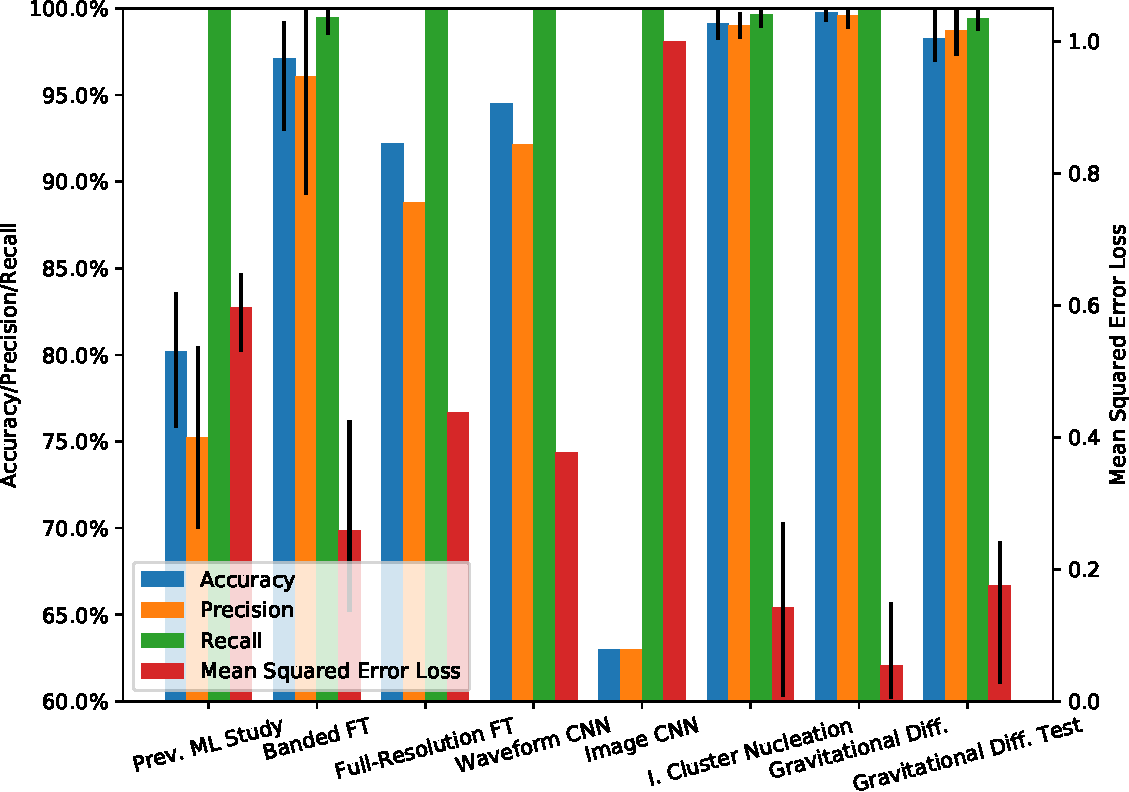
\includegraphics[width=0.85\textwidth]{pico_final_results}}
    \caption{\label{pico_final_results} Validation accuracy, precision, recall, and loss for each technique in PICO-60. Error bars represent the 8th and 92nd percentiles.}
\end{figure}

\subsection{DEAP-3600}

The three algorithms I developed were evaluated based on their reduction in the rate of false positives (simulated WIMP events misidentified as neck alphas) compared to the 91.0\% result achieved with a conventional classifier. Only models with at least 99.6\% neck alpha removal (in line with the conventional classifier) were considered.

Both the dense neural network and topological CNN produced a higher rate of false positives than the conventional classifier, meaning that they misclassified more WIMPs as alpha particles. However, as seen in Figure \ref{deap_final_results}, the cylindrical projection method \textit{reduced} the false positive rate from 91.0\% to 75.7\%.

This successful network model was tested on the limited amount of available real-world data. It removed 73.9\% of WIMP-like (neutron calibration) events, which is in line with the 75.7\% obtained on simulated data.

However, only 91.2\% of background events (expected to be neck alphas) were removed, quite far off the 99.6\% reached on simulated data. This indicates one of three possibilities:

\begin{enumerate}
    \item The simulation is not an accurate representation of the real-world detector (some physical dynamic has not been simulated), and thus the network did not generalize.
    \item There is WIMP dark matter present in the set of background events.
    \item There is an unanticipated form of background radiation present.
\end{enumerate}

\begin{figure}[ht]
    \centering
    \fbox{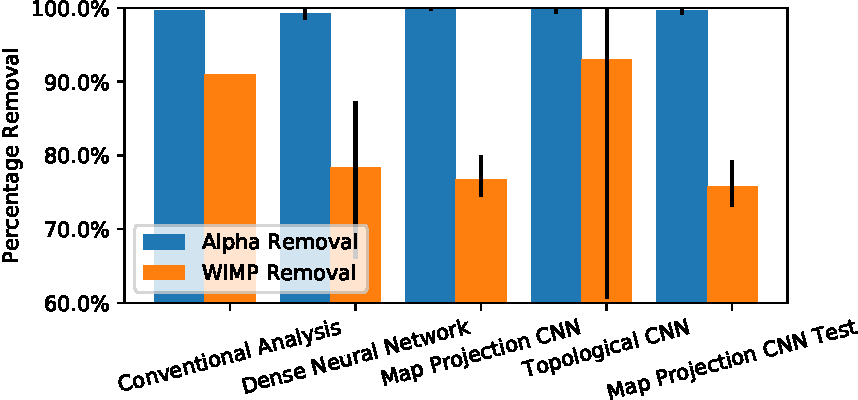
\includegraphics[width=0.5\textwidth]{deap_final_results}}
    \qquad
    \begin{tabular}[b]{|l|l|l|}
        \hline
        Method & Backgnd. & WIMP \\
        \hline
        Conventional & 99.6\% & 91.0\% \\
        \hline
        Dense NN & 100\% & 100\% \\
        \hline
        Cylindrical & 99.9\% & 76.7\% \\
        \hline
        Topological & 99.9\% & 93.0\% \\
        \hline
        Cyl Sim Test & 99.6\% & 75.7\% \\
        \hline
        Cyl Real Test & 91.2\% & 73.9\% \\
        \hline
    \end{tabular}
    \caption{\label{deap_final_results} Background and WIMP removal rates for the highest-accuracy hyperparameter configuration of each technique in DEAP-3600.}
\end{figure}

\section{Conclusion}

These results confirm that I achieved my goal. While the conventional classifier in PICO-60 is believed to be perfectly accurate, my semi-supervised learning methods have significantly improved the accuracy that can be obtained quickly and without manual optimization. This should allow physicists working on future iterations of PICO to iterate more quickly, without modifying a conventional classifier whenever some aspect of the experiment changes.

The reduction in the false positive rate for DEAP-3600 provides evidence that machine learning can improve the efficiency of this experiment, possibly reducing the operation time required to collect sufficient evidence for or against the existence of WIMP dark matter.

Additionally, the unusual predictions made on real-world data provide important diagnostic information on the DEAP-3600 simulation (assuming that WIMPs are not present).

Fundamentally, the problems I have solved are not specific to PICO-60 and DEAP-3600; they are common across many dark matter detection experiments. Thus, my algorithms are broadly applicable, and demonstrate promise in the field as a whole.

\section{Acknowledgements}

Many thanks to Dr.~Nigel~Smith, Dr.~Ken~Clark, Dr.~Carsten~Krauss, Dr.~Scott~Fallows, Dr.~Eric~V\'azquez-J\'auregui, and Dr.~Pierre~Gorel for introducing me to PICO-60 and DEAP-3600, and generously providing access to data for training.

\section{References}

\printbibliography[heading=none]

\pagebreak

\section{Bibliography}

\begin{itemize}
    \item All programming for this study was done in Python 3 \cite{python}.
    \item Keras \cite{keras}, running on a TensorFlow \cite{tensorflow} backend, was used for all machine learning tasks.
    \item NumPy \cite{numpy} and SciPy \cite{scipy} were used for linear algebra and signal processing.
    \item ROOT \cite{root}, scikit-image \cite{scikit-image}, and scikit-learn \cite{scikit-learn} were used for data loading and storage.
    \item Matplotlib \cite{matplotlib} was used for data visualization.
\end{itemize}

\end{document}